\chapter{CPU Scheduling}
L'obiettivo della multiprogrammazione è fare in modo che vi sia sempre un processo in esecuzione, al fine di massimizzare l'utilizzo della CPU.

\section{CPU e I/O Burst Cycle}
L'esecuzione di un processo consiste in un ciclo di utilizzo della CPU e attesa di operazioni di I/O. Inizia con un periodo di utilizzo della CPU (\textbf{CPU burst)}, 
seguito da un periodo di attesa per operazioni di I/O (\textbf{I/O burst}), continuando così finchè la CPU termina con una system call per concludere l'esecuzione.

\begin{figure}[!htb]
    \centering
    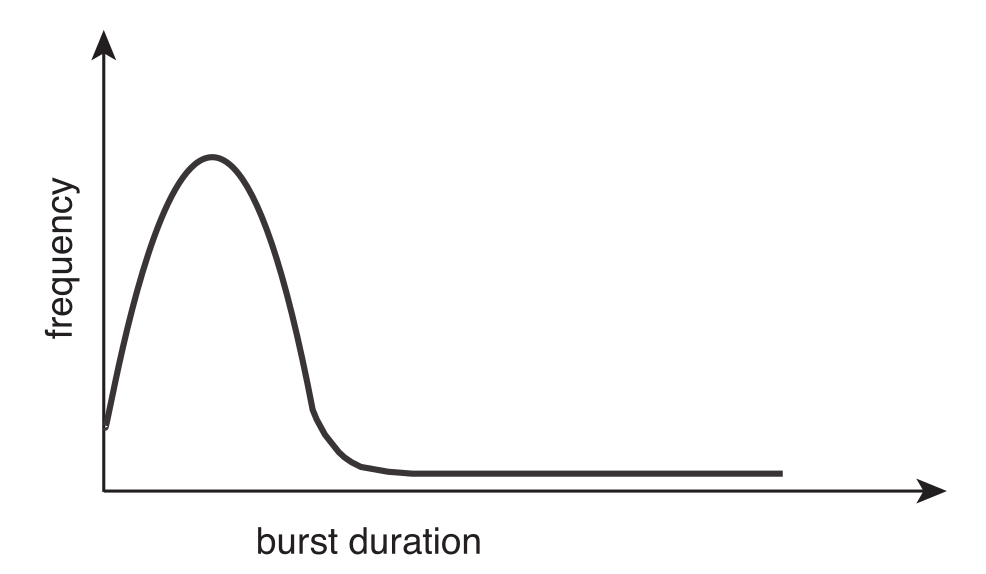
\includegraphics[width=0.5\linewidth]{Images/cpu_sched/burst.png}
    \caption{Durata del burst della CPU.}
\end{figure}

\section{CPU Scheduling}
Ogni volta che la CPU diventa inattiva, il sistema operativo deve selezionare uno dei processi nella ready queue affinché venga eseguito.
Questo compito è assegnato allo \textbf{Scheduler dello CPU}. Gli elementi contenuti in tali code sono, in genere, i blocchi di controllo del processo (PCB) dei processi stessi. \\ 
Ci possono essere quattro circostanze diverse:
\begin{enumerate}
  \item Processo passa da stato di runnig a stato di waiting.
  \item Processo passa da stato di running a stato ready.
  \item Processo passa da stato di waiting a stato ready.
  \item Processo che termina.
\end{enumerate}
Per il caso 1 e 4 lo scheduling è chiamato \textbf{nonpreemtive}, dato che non c'è nessun tipo di scelta da fare. 
Invece, nei casi 2 e 3, lo scheduling è chiamato \textbf{preemtive}.

\subsection{Dispatcher}
\begin{defn}
Componente che fa parte della funzione di scheduling della CPU. 
Questo modulo si occupa di dare il controllo del processo selezionato dallo scheduler al core disponibile.
\end{defn}
Ci sono diverse funzioni che esegue:
\begin{itemize}
  \item Cambio di contesto fra un processo e l'altro.
  \item Cambiare alla modalità utente.
  \item Saltare alla posizione corretta per riprendere l'esecuzioni di un programma.
\end{itemize}

\begin{figure}[!htb]
    \centering
    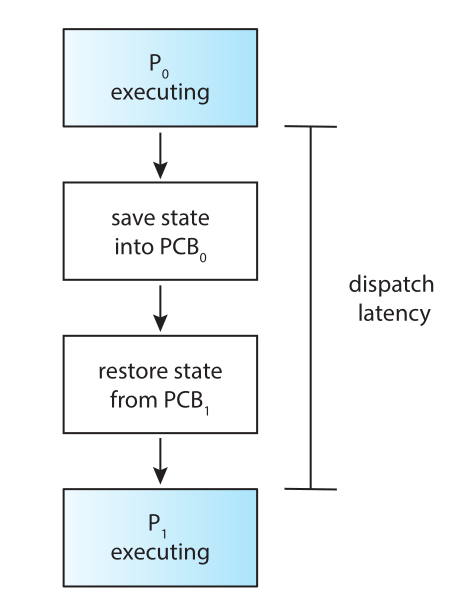
\includegraphics[width=0.3\linewidth]{Images/cpu_sched/dispatcher.png}
    \caption{Dispatcher e Latenza.}
\end{figure}

Deve essere molto veloce e efficente, dato che deve essere chiamato a ogni context swicth. \\ 
Il tempo che impiega il dispatcher è chiamato \textbf{latenza del dispatcher}.

\subsection{Criteri di Scheduling}
Ci sono numerosi algortimi di scheduling, ognuno che migliora e ottimizza diversi aspetti. Per confrontarli, è necessario avere dei criteri precisi:
\begin{itemize}
  \item \textbf{Utilizzo della CPU:} mantenere la CPU più occupata possibile.
  \item \textbf{Throughput:} massimizzare il numero di processi che completano la propria esecuzione per unità di tempo.
  \item \textbf{Tempo di esecuzione:} minimizzare il tempo totale di esecuzione di un processo (ready queue + i/o and cpu time).
  \item \textbf{Tempo di waiting:} minimizzare il tempo che un processo rimane nella ready queue.
  \item \textbf{Tempo di risposta:} minimizzare il tempo il tempo che il processo ci mette, dopo essere stato eseguito, a dare la prima risposta.
\end{itemize}

In base al tipo di utilizzo, si può cercare di ottimizzare alcuni criteri rispetto ad altri. \\
Per esempio, un computer consumer, dovrà preferire velocità e fluidità nell'utilizzo di interfaccie e programmi. In un server, invece, potrebbe essere necessario ottimizzare il throughput, dato che non ha bisogno di interfaccie grafiche fluide.

\newpage
\section{Algortimi di Scheduling}
In questa parte verrano analizzati i principali algortimi di scheduling. 
In questa prima parte, viene considerato il caso in cui la CPU abbia un solo core, potendo eseguire un solo processo alla volta.

\subsection{First-Come, First-Served (FCFS)}
Algortimo più semplice, viene gestito tramite una coda FIFO. Quando un processo viene inserito nella ready queue, il suo PCB viene aggiunto in coda.
Quando la CPU è libera viene eseguito il primo processo della coda.

\begin{center}
    \begin{tabular}{c@{\hspace{2cm}}c}
        \underline{Process} & \underline{Burst Time} \\[4pt]
        $P_1$              & 24                     \\
        $P_2$              & 3                      \\
        $P_3$              & 3
    \end{tabular}
\end{center}

\begin{figure}[!htb]
    \centering
    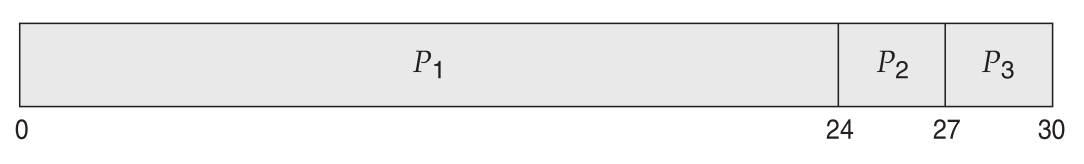
\includegraphics[width=0.5\linewidth]{Images/cpu_sched/fcfs.png}
    \caption{Gaant FCFS.}
\end{figure}

Questo metodo è nonpreemtive, quindi una volta che un processo viene asseganto alla cpu, finisce di eseguire. Questo è particolarmente scomodo in sistemi interattivi, in cui ogni processo ha una fetta di tempo di cpu.
Inoltre, nel caso il primo processo sia quello più lungo, potrebbe aumentare sostanzialmente il tempo medio di wait, risultando in un utilizzo della cpu poco efficente.

\subsection{Shortest-Job-First (SJF)}
In questo algoritmo, a ogni processo viene assegnato il tempo di cpu burst. Quando la cpu diventa libera, viene mandato in esecuzione il processo con il tempo minore.

\begin{center}
    \begin{tabular}{c@{\hspace{2cm}}c}
      \underline{Process} & \underline{Burst Time} \\[4pt]
        $P_1$ & 6 \\
        $P_2$ & 8 \\
        $P_3$ & 7 \\
        $P_4$ & 3
    \end{tabular}
\end{center}

\begin{figure}[!htb]
    \centering
    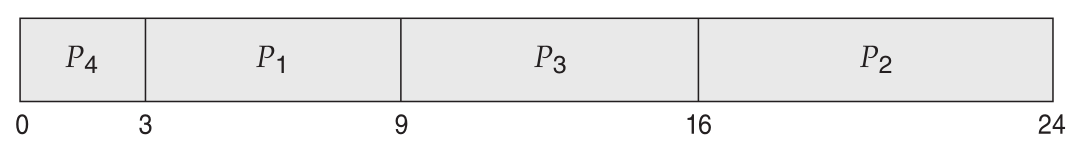
\includegraphics[width=0.5\linewidth]{Images/cpu_sched/sjb.png}
    \caption{Gaant SJB.}
\end{figure}

Se due processi avranno un burst time uguale, allora si usa fra di loro la metodologia FCFS. \\ 
Questo algortimo sarebbe ottimale, ma non è implementabile, visto che non si può sapere a priori quale sarà il tempo di burst. L'unico modo è provare a prevederlo.
Il prossimo tempo di burst della cpu è predetto attarverso una \textbf{media esponenziale}, utilizzando il burst precedente:
\[
  \tau_{n+1} = \alpha t_n + (1 - \alpha)\tau_n
\]
Dove:
\begin{itemize}
  \item $0 \ge \alpha \ge 1$.
  \item $t_n$ è il burst precedente.
  \item $\tau_n$ contiene tutti i valori passati.
  \item $\tau_{n+1}$ è il tempo che vogliamo predirre.
\end{itemize}
Se $\alpha$ è uguale a 0, allora la storia passata non ha importanza, invece, se $\alpha$ è uguale a 1, allora ha importante solo il burst più recente. \\ 
Solitamente, come valore di $\alpha$ viene utilizzato $\frac{1}{2}$ e come valore di $\tau_0$ viene utilizzata una costante o la media generale del sistema.

\newpage
\begin{figure}[!htb]
    \centering
    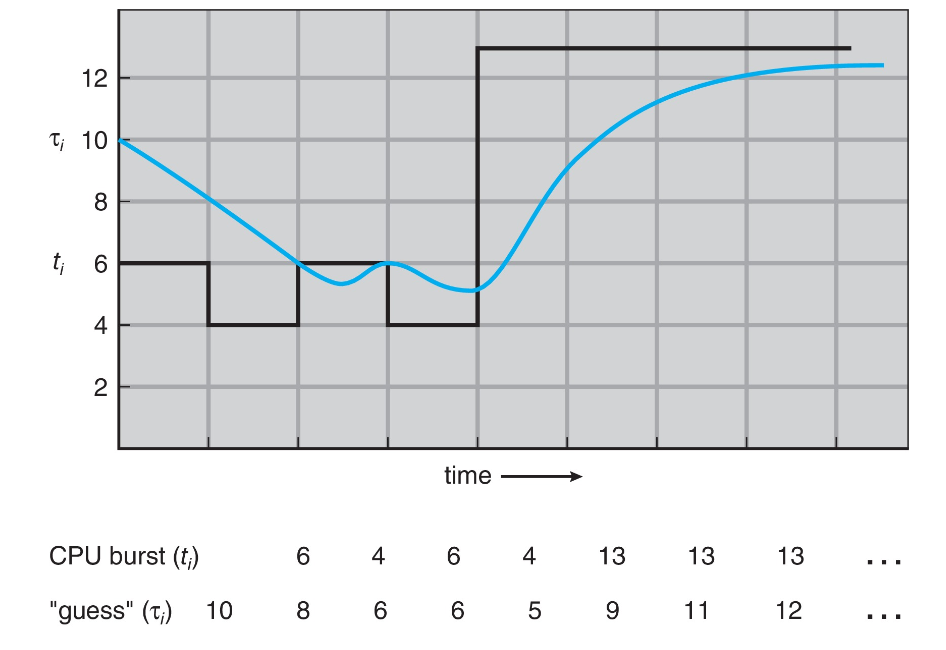
\includegraphics[width=0.5\linewidth]{Images/cpu_sched/prediction.png}
    \caption{Prediction burst SJB.}
\end{figure}

In questo caso con i valori $\alpha = \frac{1}{2}$ e $\tau_o = 10$, si può raggiungere una buona approssimazione. \\ 
Questo algortimo può essere sia non nonpreemtive che preemtive, nel caso i processi abbiamo un burst di cpu minore del tempo totale che gli serve. 
Quest'ultimo caso è anche chiamato \textbf{shortest-remaining-time-first}.

\subsection{Round-Robin (RR)}
Questo algortimo è simile al FCFS, ma è preemtive, permettendo al sistemi di cambiare processi.
L'implemntazione richiede l'utilizzo di una piccola unità di tempo chiamata \textbf{time quantum} o \textbf{time slice}. \\ 
Nello specifico, la coda ready viene trattata come se fosse circolare e lo scheduler esegue per un quantum time ogni processo, uno dopo l'altro. 
Anche in questo caso la ready queue è trattata come FIFO, quindi i nuovi processi vengono aggiunta alla fine. Le situazioni possibili sono due:
\begin{enumerate}
  \item Il processo dura meno di un quantum time, quindi termina e si passa a quello successivo.
  \item Il processo dura di più di un quantum time, quindi quando il timer finisce, processo corrente viene inserito alla fine della coda, viene lanciata una interrupt al sistema operativo e viene eseguito un cambio di contesto al processo successivo.
\end{enumerate}

\begin{center}
    \begin{tabular}{c@{\hspace{2cm}}c}
        \underline{Process} & \underline{Burst Time} \\[4pt]
        $P_1$              & 24                     \\
        $P_2$              & 3                      \\
        $P_3$              & 3
    \end{tabular}
\end{center}

Ipotizziamo un quatum time $q$ uguale a $4 ms$. Il processo $P_1$ viene eseguito per 4 millisecondi, poi interrotto. Dopo il cambio di contesto viene eseguito $P_2$ che termina. Per $P_3$ stessa situazioni. Infine, rimane da eseguire il processo $P_1$.

\begin{figure}[!htb]
    \centering
    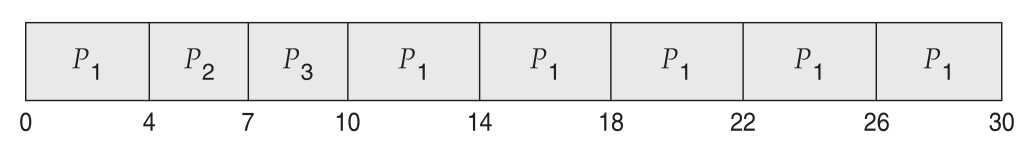
\includegraphics[width=0.5\linewidth]{Images/cpu_sched/rr.png}
  \caption{Gaant RR.}
\end{figure}

Se il quatum time è molto elevato, questo algortimo si trasforma in un FCFS, invece, se molto piccolo, potrebbe richiedere un numero molto grande di cambi di contesto. 
Solitamente, l'80\% del tempo di burst deve essere inferiore al quatum time per ottenere un buon risultato.

\begin{figure}[!htb]
    \centering
    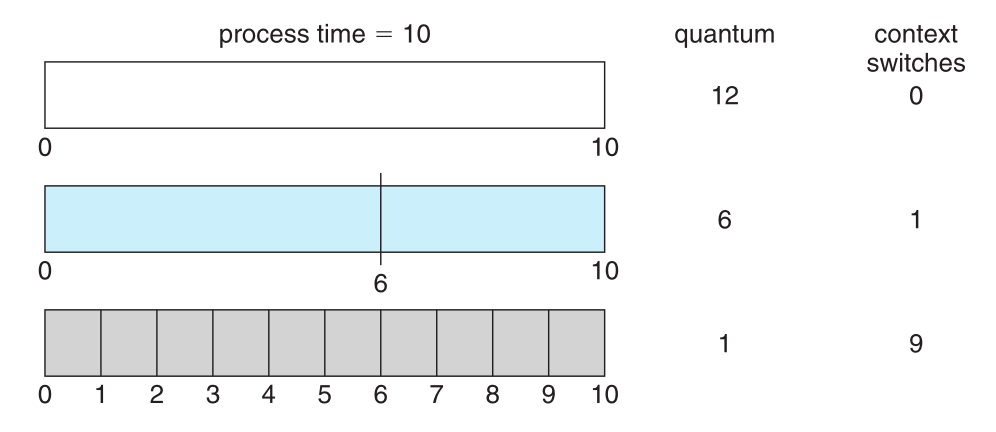
\includegraphics[width=0.35\linewidth]{Images/cpu_sched/quantum.png}
  \caption{Esempio di scelte del quatum time.}
\end{figure}

\subsection{Scheduling con Priorità}
L'algortimo SJF era una caso specifico del più generale algortimo di scheduling con priorità.
A ogni processo viene assegnata un priorità, quello con il valore maggiore viene scelto per essere eseguito sulla cpu. In caso di priorità uguale viene sempre usata la metodologia di FCFS.

\begin{center}
    \begin{tabular}{c@{\hspace{2cm}}c@{\hspace{2cm}}c}
      \underline{Process} & \underline{Burst Time} & \underline{Priority} \\[4pt]
      $P_1$ & 10 & 3 \\
      $P_2$ & 1 & 1 \\
      $P_3$ & 2 & 4 \\
      $P_4$ & 1 & 5 \\
      $P_5$ & 5 & 2
    \end{tabular}
\end{center}

\begin{figure}[!htb]
    \centering
    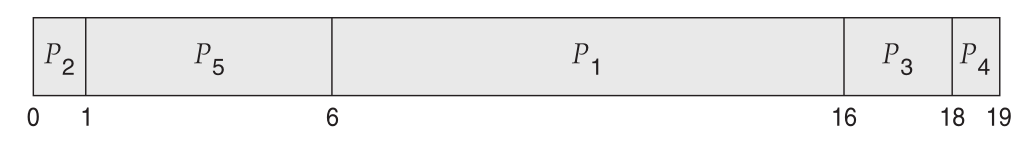
\includegraphics[width=0.5\linewidth]{Images/cpu_sched/priority.png}
  \caption{Gaant Scheduling con Priorità.}
\end{figure}

Le priorità possono essere assegnate internamente, usando informazioni come burst di I/O, burst di CPU, file aperti, memoria, ecc...
Alternativamente, possono essere assegnate esternamente, per esempio in base all'importanza del processo. Questo algortimo può essere sia preemtive che nonpreemtive. \\ 
\vspace*{0.01\textheight}
Questo algortimo, però, introduce un problema: la \textbf{starvation}. Si verifica quanto un processo della ready queue a priorità bassa non viene mai eseguito,
questo è probabile in sistemi complessi in cui sono presenti numerosi processi con priorità più alta. Un soluzione adottata è quella dell'\textbf{aging}.
I processi nella coda di ready possono aumentare la priorità in base al tempo in cui rimangono pronti.

\section{Scheduling Code Multilivello}
Se si usa un algortimo di round robin con una coda a priorità, per trovare i processi con priorità si ha una complessita $O(n)$. 
Una strategia per ridurre la complessità può essere quella di creare più code, ognuna associato un numero di priorità.

\begin{figure}[!htb]
    \centering
    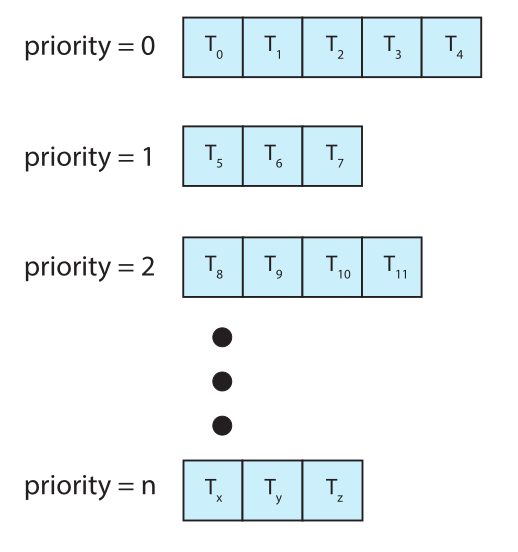
\includegraphics[width=0.3\linewidth]{Images/cpu_sched/multiqueue.png}
  \caption{Code di Priorità.}
\end{figure}

Questo meccanismo permette di dividere i processi in diverse categorie, per esempio, \textit{background} e \textit{foreground}, oppure dividendoli in processi \textit{real time}, di \textit{sistema}, \textit{interattivi}, ecc...

\section{Thread Scheduling}
Nelle sezioni precedenti era stata specificata la differenza fra \textbf{kernel thread} e \textbf{user thread}. I kernel thread vengono gestiti dal sistema operativo, invece, gli user thread sono gesiti da librerie utente.
Per il collegamento fra i due tipi di thread sarà necessario avere un processo molto leggero (\textbf{LWP}).

\subsection{Contention Scope}
I modelli di gestione dei thread come many-to-many e many-to-one, la libreria dei thread gestisce quali thread assegnare all'LWP, conosciuto anche come \textbf{Process-Contention Scope} (\textbf{PCS}), dato che i thread devono competere fra di loro.
Il meccanismo di scheduling del thread su un core fisico, si chiama \textbf{System-Contention Scope} (\textbf{SCP}). \\ 
Nel caso di modelli one-to-one, il sistema di PCS non viene usato, ma si usa solo il PCS, dove tutti i thread competono fra di loro.

\subsubsection{Pthread Scheduling}
L'API POISX di \texttt{Pthread}, permette di usare entrambi le metodologie:
\begin{itemize}
  \item \textbf{PCS Scheduling:} in \texttt{Pthread} si può usare con il valore \texttt{PTHREAD\_SCOPE\_PROCESS}.
  \item \textbf{SCP Scheduling:} in \texttt{Pthread} si può usare il valore \texttt{PTHREAD\_SCOPE\_SYSTEM}
\end{itemize}

\begin{clang}[Esempio in C per conper controllare lo SCOPE]
#include <pthread.h>
#include <stdio.h>
#define NUM_THREADS 5

int main(int argc, char *argv[]) {
  int i, scope;
  pthread_t tid[NUM_THREADS];
  pthread_attr_t attr;

  /* get the default attributes */
  pthread_attr_init(&attr);
  
  /* first inquire on the current scope */
  if (pthread_attr_getscope(&attr, &scope) != 0)
    fprintf(stderr, "Unable to get scheduling scope\n");
  else {
    if (scope == PTHREAD_SCOPE_PROCESS)
      printf("PTHREAD_SCOPE_PROCESS");
    else if (scope == PTHREAD_SCOPE_SYSTEM)
      printf("PTHREAD_SCOPE_SYSTEM");
    else
      fprintf(stderr, "Illegal scope value.\n");
  }

  /* set the scheduling algorithm to PCS or SCS */
  pthread_attr_setscope(&attr, PTHREAD_SCOPE_SYSTEM);

  /* create the threads */
  for (i = 0; i < NUM_THREADS; i++)
    pthread_create(&tid[i],&attr,runner,NULL);

  /* now join on each thread */
  for (i = 0; i < NUM_THREADS; i++)
    pthread_join(tid[i], NULL);
}

/* Each thread will begin control in this function */
void *runner(void *param)
{
  /* do some work ... */
  pthread_exit(0);
}
\end{clang}

\section{Scheduling per Processi Multipli}
Nella prima parte è stato trattato lo scheduling su single-core, 
invece, sopratutto in sistemi moderni, i sistemi presentano più corse fisici, rendendo più complesso lo scheduling.

\subsection{Approcci allo Scheduling di Processi Multipli}
Un primo approccio usato, chiamato \textbf{Multiprocessing Asimetrico}, è quello di dedicare un solo core per le decisioni di scheduling, gestione dell'I/O e altre attività del sistema.
Gli altri core eseguono solo il codice dell'utente. Questo, però, può potenzialmente creare un bottlenck. \\ 
Nei sistemi moderni si è passato a un approccio diverso, ossia \textbf{Multiprocessing Simmetrico} (\textbf{SMP}), dove ogni core si auto schedula.
Ogni processo, in questo caso, hai il suo scheduler che seleziona da una coda di thread pronti, creando due situazioni diverse:
\begin{enumerate}
  \item Una coda unica globale con tutti i thread.
  \item Una coda di thread privata per ogni processo.
\end{enumerate}

\begin{figure}[!htb]
    \centering
    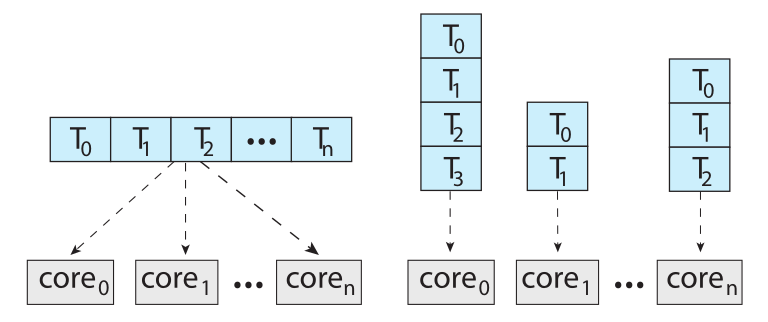
\includegraphics[width=0.5\linewidth]{Images/cpu_sched/coda-thread.png}
  \caption{Esempio delle due situazioni.}
\end{figure}

Il primo scenario, potrebbe a sua volta creare un bottleneck, quindi, normalmente è usato sempre il secondo.

\subsection{Processori Multicore}
In sistemi moderni, invece di avere più processori, si è passato ad avere più core nello stesso processore. Permette di essere più veloce e più efficente. \\ 
Un problema però, dato che i processori hanno velocità molto elevate, aspettano quasi la metà del tempo ad aspettare le memorie, questo tempo è chiamato \textbf{memory stall}.

\begin{figure}[!htb]
    \centering
    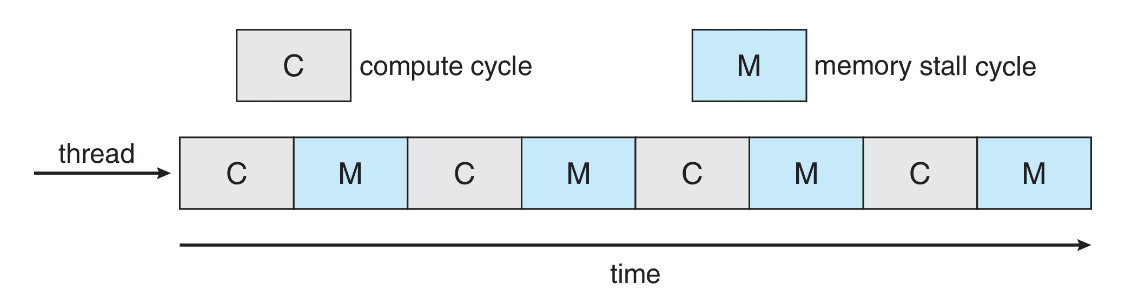
\includegraphics[width=0.5\linewidth]{Images/cpu_sched/stall.png}
  \caption{Esempio con Memory Stall.}
\end{figure}

Una soluzione è usare sempre più di un thread, così nel caso uno abbia un memory stall, si sempre l'altro.

\begin{figure}[!htb]
    \centering
    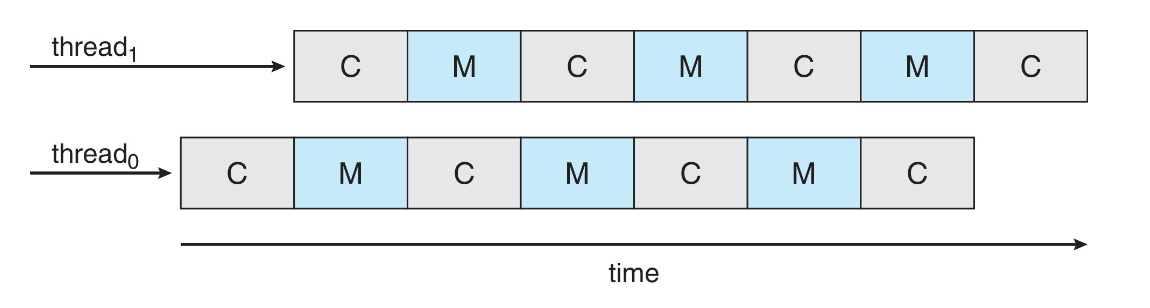
\includegraphics[width=0.5\linewidth]{Images/cpu_sched/stall-sol.png}
  \caption{Esempio con Memory Stall e più Thread.}
\end{figure}

Questa tecnica è chiamata \textbf{Chip Multithreading} (\textbf{CMT}). Per esempio, un processore con 4 core, di cui ognuno ha 2 thread, agli occhi del sistema operativo avrà 8 CPU.
Esitono due tipi:
\begin{enumerate}
  \item \textbf{Coarse-Grained:} un core esegue finchè non incontra un evento molto come un memory stall. Quando succede, si cambia a un nuovo thread che inizia l'esecuzione.
    Cambiare i thread richiede di svutare la pipeline ed è quindi molto costoso.
  \item \textbf{Fine-Grained:} cambiano i thread con un grado più fino, vicino al confine di un ciclo di istruzione, aggiungendo una logica di thread switching.
    Questo metodo aggiunge un costo piccolo.
\end{enumerate}

\begin{note}[NOTA BENE]
Le risorse come cache e pipeline, sono condivise fra tutti gli hardware thread, dei quali ne può essere eseguito solo uno alla volta.
Servono, quindi, due livelli di decisione:
\begin{enumerate}
  \item Primo livello in cui il sistema operativo decide quali thread software devono girare sui thread hardware.
  \item Secondo livello in cui viene deciso quale thread hardware deve essere eseguito.
\end{enumerate}
\end{note}

\begin{figure}[!htb]
    \centering
    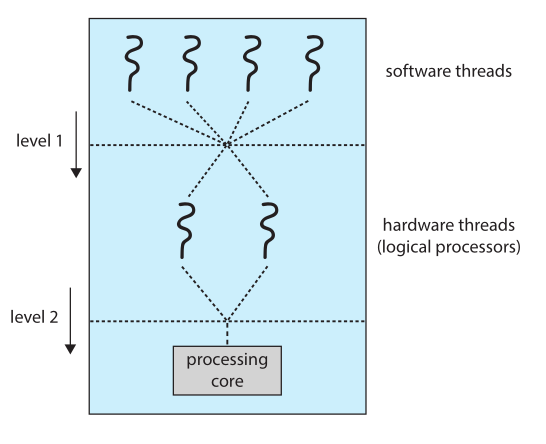
\includegraphics[width=0.4\linewidth]{Images/cpu_sched/thread-level.png}
  \caption{Esempio di Multithreading.}
\end{figure}

\begin{defn}[Load Balancing]
Nei sistemi multicore simmetrici, per sfruttare al meglio e in modo efficente tutti i core, per evitare che alcuni siano in idle e altri con le code piene, è necessario un \textbf{load balancer}.
Ci sono due approcci diversi:
\begin{enumerate}
  \item \textbf{Push Migration:} un task controlla periodicamente i core, nel caso uno sia sovraccaricato, sposta i thread in un core idle e meno occupato.
  \item \textbf{Pull Migration:} un core idle prende thread da core più occupati o sovraccaricati.
\end{enumerate}
\end{defn}

\section{Scheduling della CPU in Real Time}
Lo scheduling per sistemi real time richiede qualche accortezza in più. In generale, però, possiamo dividerli in due categorie:
\begin{enumerate}
  \item \textbf{Soft Real-Time Systems:} i processi critici hanno priorità maggiore, ma non si sa quando verranno eseguiti.
  \item \textbf{Hard Real-Time Systems:} i processi \textcolor{red}{\textbf{devono}} essere eseguiti prima della loro deadline.
\end{enumerate}

\subsection{Minimizzare la Latenza}
I sistemi real time sono basati tipicamente su eventi, quindi quando ricevono una richiesta, è necessario che rispondano nel minor tempo possibile.
Il tempo passato da quanto accade un evento e quando viene servito è chiamato \textbf{latenza dell'evento}. Questo tempo può cambiare per molti fattori, tra cui:
\begin{itemize}
  \item \textbf{Latenza di Interrupts:} tempo passato fra l'arrivo di una interrupt e l'inizio della sua routine.
  \item \textbf{Latenza di Dispatch:} tempo usato dal dispatcher per cambiare dal processo corrente a un altro processo. 
    In questa latenza, potrebbe pure esserci una fase di conflitto, nel caso sia preemtive.
\end{itemize}

\subsection{Scheduling Basato su Priorità}
La parte più importante nei sistemi real time è rispondere velocemente, quindi devono poter avere uno scheduling con priorità e preemtive. Questo garantisce sicuramente che il sistema sia almeno soft real-time. \\
Per i sistemi hard real-time, invece, deve essere garantito che finiscano entro la loro deadline. \\ Prima di capire i var algortimi, è necessario capire le caratteristiche di ogni processo:
\begin{enumerate}
  \item I processi sono \textbf{periodici}. Richiedono la CPU a intervalli di tempo $p$.
  \item Ogni processo a un tempo di fissato di esecuzione $t$.
  \item Ogni processo ha una deadline $d$ entro qui deve essere completato.
  \item Il \textbf{rate} di una task periodica è $\frac{1}{p}$.
\end{enumerate}
La relazione fra questi valori è:
\[
  0 \le t \le d \le p
\]
Ogni processo, però, deve annunciare allo scheduler il suo tempo di deadline, permettendo allo scheduler due scelte: accettarlo o rifiutarlo, nel caso non possa garantire l'esecuzione entro la deadline.

\subsection{Rate-Monotic Scheduling (RMS)}
In questo algortimo, la priorità è inversamente proporzionale al periodo. Più il periodo è corto, maggiore è la priorità. Questo favorisce i processi che richiedono spesso la CPU per poco tempo.

\begin{figure}[!htb]
    \centering
    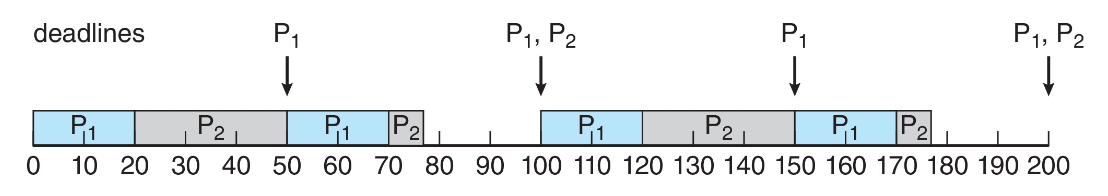
\includegraphics[width=0.5\linewidth]{Images/cpu_sched/rms.png}
  \caption{Esempio con priorità di P1 magiore di P2.}
\end{figure}

Alcune volte, però, potrebbe capitare che i processi non finiscano entro la loro deadline.

\subsection{Ealiest Deadline First Scheduling (EDF)}
In questo algortimo la priorità viene assegnata in modo dinamico in base alla deadline, prima è più sarà alta la priorità. \\ 
Ogni processo deve annunciare al sistema la propria deadline, dopo le priorità verranno aggiustate in base al nuovo processo.

\begin{figure}[!htb]
    \centering
    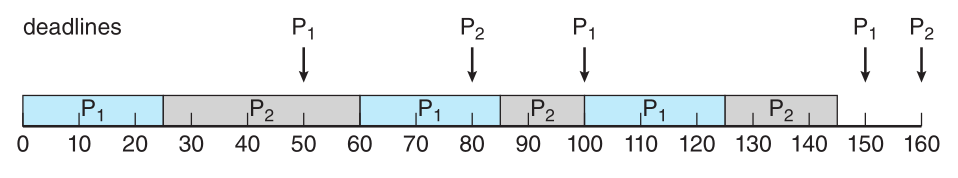
\includegraphics[width=0.5\linewidth]{Images/cpu_sched/edf.png}
  \caption{Esempio di Algortimo EDF.}
\end{figure}

\subsection{Proportional Share Scheduling (PSS)}
In questo algortimo alloca $T$ parti fra tutte le applicazioni. Successivamente, un'applicazione può chiedere $n$ parti, avendo quindi $\frac{N}{T}$ del tempo totale del processore. \\ 
Aggiungendo delle regole di ammissione e controllo, si riesce a garantire ai processi le parti necessarie per eseguire completamente.

\subsection{Scheduling Real-Time POSIX}
All'interno dell'API standard esistono due tipi di classi che permettono l'implementazione di thread real-time:
\begin{itemize}
  \item \texttt{SCHED\_FIFO}: usa una coda FIFO, il primo che entra è il rpimo che esegue.
  \item \texttt{SCHE\_RR}: usa un algortimo round-robin che garantisce parti di tempo a ogni task.
\end{itemize}
Tramite due funzioni è possibile impostare un di queste di policy:
\begin{enumerate}
  \item \texttt{pthread\_attr\_getsched\_policy(pthread\_attr\_t *attr, int *policy)}.
  \item \texttt{pthread\_attr\_getsched\_policy(pthread\_attr\_t *attr, int *policy)}.
\end{enumerate}


\begin{clang}[Esempio di Scheduling Real-Time POSIX]
#include <pthread.h>
#include <stdio.h>
#define NUM_THREADS 5
int main(int argc, char *argv[])
{
  int i, policy;
  pthread_t tid[NUM_THREADS];
  pthread_attr_t attr;

  /* get the default attributes */
  pthread_attr_init(&attr);

  /* get the current scheduling policy */
  if (pthread_attr_getschedpolicy(&attr, &policy) != 0)
    fprintf(stderr, "Unable to get policy.\n");
  else {
    if (policy == SCHED_OTHER) printf("SCHED_OTHER\n");
    else if (policy == SCHED_RR) printf("SCHED_RR\n");
    else if (policy == SCHED_FIFO) printf("SCHED_FIFO\n");
  }

  /* set the scheduling policy - FIFO, RR, or OTHER */
  if (pthread_attr_setschedpolicy(&attr, SCHED_FIFO) != 0)
    fprintf(stderr, "Unable to set policy.\n");
  
  /* create the threads */ for (i = 0; i < NUM_THREADS; i++)
  pthread_create(&tid[i],&attr,runner,NULL);

  /* now join on each thread */ for (i = 0; i < NUM_THREADS; i++)
  pthread_join(tid[i], NULL);
}

/* Each thread will begin control in this function */
void *runner(void *param){
  /* do some work ... */
  pthread_exit(0);
}
\end{clang}
